\chapter{Modélisation et analyse des premières opérations de chaque pièce}
Maintenant que nous connaissons un modèle valide pour une opération ainsi que les temps nécessaires au déplacement du chariot sur l'axe vertical et horizontal, nous allons pouvoir commencer à modéliser le travail du \emph{STA} sur deux opérations.

Nous allons, dans un premier temps, effectuer une modélisation en RdP Temporels d'une commande de deux opérations suite à quoi, nous en effectuerons une analyse grâce à une version de \emph{TINA} identique que dans le chapitre \ref{chap:realisationUneOperation}. Nous utiliserons cette analyse pour déterminer les intervalles d'attentes et le meilleur ordonnancement possible pour ne pas déclencher l'alarme.

\section{Réseau de PETRI Temporels de commande de deux opérations}
A partir du modèle générique établit en \ref{sec:modelGenerique}, nous avons obtenu, pour la commande de opérations $O_1$ et $O_2$ le modèle RdP Temporels en figure \ref{fig:command2Opes}.
\begin{figure}
\centering
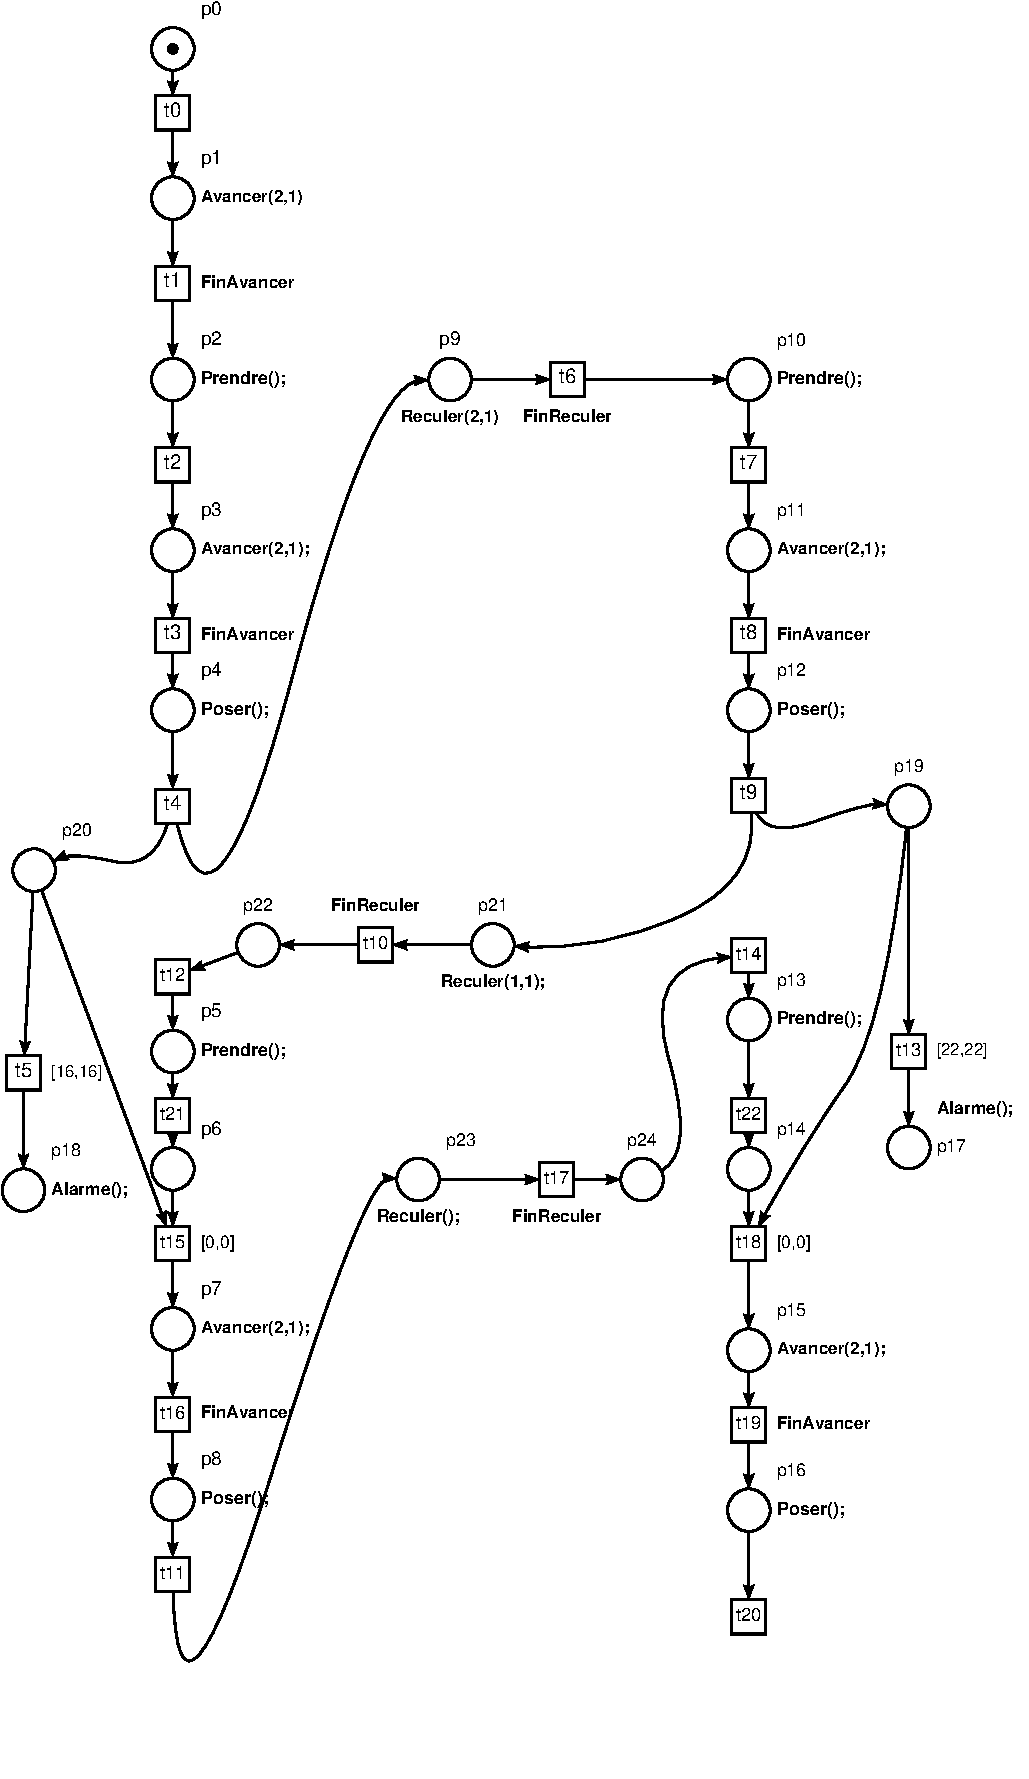
\includegraphics[height = \textheight]{./II/images/reseau_CommandeIII-2.pdf}
\caption{Réseau de PETRI Temporels pour la commande de 2 opérations}\label{fig:command2Opes}
\end{figure}

Dans ce réseau, nous pouvons identifier tout d'abord la ressemblance avec le modèle générique (en figure \ref{fig:RdPTempo_generique}) : les places $p_4$ et $p_{12}$ sont les représentations de la place $p_2$ dans le modèle générique. Elles seront donc suivi, dans les modèle Temporels que nous analyseront, d'une transition qui contient le temps des opérations \emph{Poser}. Il en va de même pour les places $p_2$, $p_{10}$, $p_{5}$ et $p_{13}$ qui contiennent l'opération \emph{Prendre}, elles seront suivi d'une transition contenant une intervalle de temps $y$.

\paragraph*{Séparation du modèle}
Nous pouvons séparer ce modèle complexe en deux ensembles de places : \begin{itemize}
\item l'ensemble $P_1 =\left\lbrace p_2,p_3,p_4,p_5,p_6,p_7,p_{20},p_{18}\right\rbrace$ est utilisé pour emmené la pièce $p1$ du bac $e1$(son bac initial) vers le bac $e3$ dans lequel elle subit l'opération $O_2$. Cet ensemble est lié avec les deux places $p_{20}$ et $p_{18}$ qui modélisent l'alarme liée à l'opération $O_1$.
\item  l'ensemble $P_2 =\left\lbrace p_{10}, p_{11}, p_{12} p_{13}, p_{14}, p_{15}, p_{16}\right\rbrace$ modélise le transport de la pièce $p2$ de $e2$(son bac initial) vers $e3$, bac dans lequel elle subit l'opération $O1$, puis du transport de $e5$ vers $e7$ (Pour prévoir les prochains RdP). L'alarme de l'opération est enclenchée par la place $p_{17}$, qui est lié au reste de l'ensemble $P_2$ par la place $p_{19}$.
\end{itemize}
	
\paragraph*{Liaison entre les ensembles}
Les places $p_9$, $p_{21}$ et $p_{23}$, places qui se situent entre les deux ensembles $P_1$ et $P_2$, sont utilisées pour effectuer les passages entre les 2 ensembles. De même, nous avons deux places $p_{22}$ et $p_{24}$ qui font la liaison entre les deux ensembles, à l'attention que celles ci ne servent pas à amener la chariot d'une pièce à l'autre mais à le faire attendre le temps nécessaire avant la fin d'une opération et donc la récupération d'une pièce.


Nous notons aussi les transitions $t_{15}$ et $t_{20}$ qui sont les représentations de la transition $t_5$ dans le modèle générique. Elles permettent dans ce contexte de synchroniser la prise de la pièce et l'arrêt du compteur de l'alarme. Comme dans le modèle générique, ces transitions ont un intervalle de temps $[0;0]$, cela oblige les jetons arrivant dans les places en amont à être immédiatement tiré. Ainsi, le compteur de l'alarme est stoppé après $0$u.t. que la pièce ait été retiré de son emplacement.

\paragraph*{Ordonnancement}
Il est aussi a noté que nous avons choisi d'effectuer l'opération de la pièce $p1$ avant celle de $p2$ et cela pour des raisons temporelles. Nous avons remarqué, dans une étude préliminaire à la construction de ce réseau, que cet ordonnancement était possible alors qu'une inversion l'ordre du traitement des pièces donne obligatoirement le retentissement d'une alarme (notamment dans la suite du TP).


Nous avons maintenant à notre disposition une commande à appliquer sur les \emph{STA}. Toutefois, avant de passer à l'implémentation, nous allons utiliser l'outil \emph{TINA} pour analyser le modèle ainsi obtenu.	


\section{Analyse du modèle avec TINA}
L'analyse temporelle de réseau nécessite un réseau tel que nous vous présentons en figure \ref{fig:RdpAnalyseIII-2}. Dans ce type de réseau, nous avons choisi de ne plus utiliser des noms sur les évènements mais plutôt des intervalles de temps. Ces intervalles ont été établi dans la section \ref{sec:estimationTemps}.

\begin{figure}[!ht]
\centering
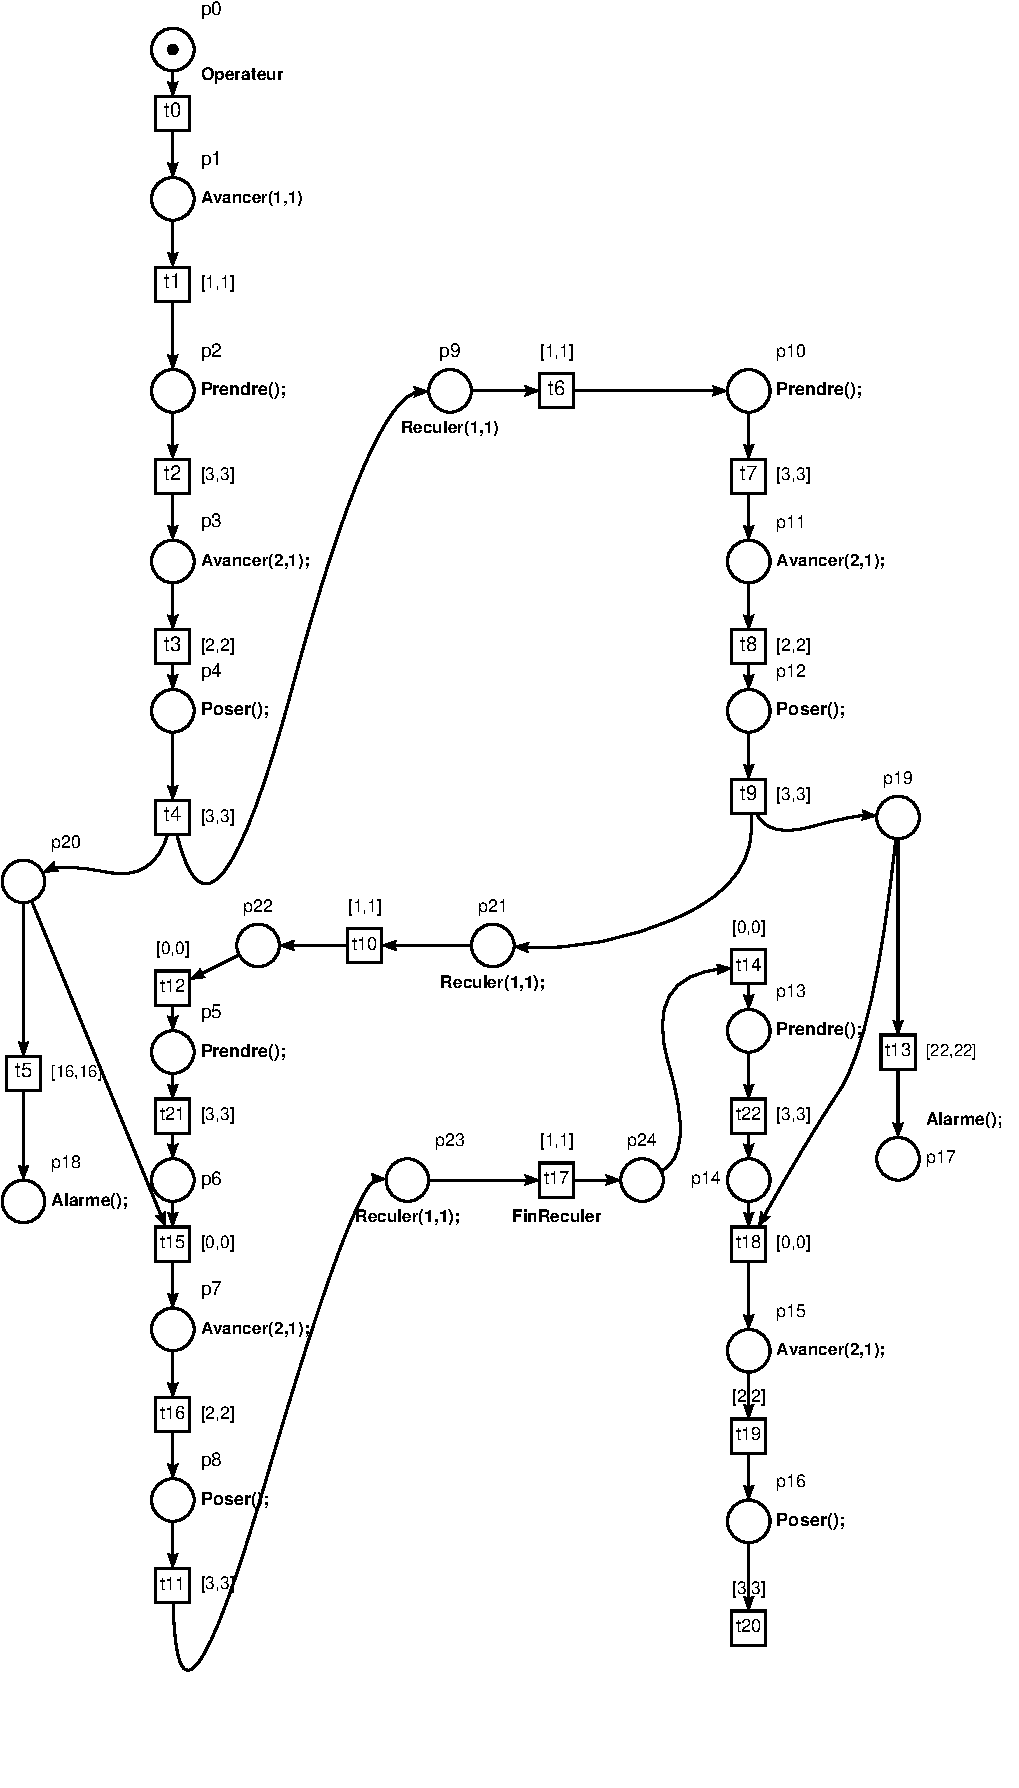
\includegraphics[height = .78\textheight]{./II/images/reseau-AnalyseIII-2.pdf}
\caption{Réseau de PETRI Temporels pour l'analyse de 2 opérations}\label{fig:RdpAnalyseIII-2}
\end{figure}

Avec la version de \emph{TINA} adéquate, nous avons réalisé la construction d'un graphe des classes accessibles. Ce graphe comporte 22 classes que nous n'avons pas représenté graphiquement, cependant vous pouvez trouver le rapport d'analyse du logiciel en annexe \ref{Annex:analyse}. 

\paragraph*{Vivacité du réseau} Dans cette analyse, nous nous referons dans un premier temps à cette bonne propriété. En effet, le résultat obtenu (disponible à la ligne 244) nous indique que les 2 transitions $t_5$ et $t_{13}$ ne sont jamais franchi. Ceci signifie que les places $p_{18}$ et $p_{17}$ ne sont jamais marqué, car le seul moyen existant pour qu'un jeton soit dans ces places est en franchissant respectivement cette transition. Donc, l'alarme n'est jamais activée.

\paragraph*{Graphe des classes}Une analyse des places accessibles à partir du graphe des classes nous confirme ce que la vivacité du réseau nous avait indiqué : les places $p_{18}$ et $p_{17}$ ne sont jamais marquées. 

Cette analyse nous apporte aussi une information que nous pourrons utiliser dans la prochaine section. Il s'agit de l'intervalle temporelle restante avant le franchissement des transitions $t_5$ et $t_{13}$ avec lequel il est possible de connaitre l'intervalle temporelle passée dans l'opération $O_1$ et $O_2$, respectivement. Nous pouvons observer aux lignes 153 et 194 ces intervalles, elles sont de $[3;3]$ pour $t_3$ et de $[9;9]$ pour $t_{13}$. 

\paragraph*{Intervalles de temps des opérations} Intéressons nous maintenant au temps d'exécution des opérations. En regardant les intervalles de temps que doivent respecter $O_1$ et $O_2$, nous pouvons connaitre le minimum et le maximum de temps admis pour les opérations. De plus, nous avons à notre disposition le temps passé dans les opérations à l'aide des transitions $t_3$ et $t_{13}$, en regardant dans le graphe des classes les intervalles de temps durant lesquelles elles peuvent être franchies. 

Donc, si l'intervalle temporelle des transitions atteint $d_{i_{max}} - d_{i_{min}}$u.t, alors la pièce doit être sorti du bac. Nous allons donc, dans la prochaine section, faire en sorte que les dernières intervalles temporelle atteinte pour $t_3$ et $t_{13}$ soit comprises entre : $[0;d_{i_{max}} - d_{i_{min}}]$.

%--> On sait le temps des opé min max
%--> On connait alors le temps des opé (dispo sur les intervalles restant de t13 et t9) 
%--> On doit obtenir le max-min sur les lignes 153 et 194

\section{Mise au point des Intervalles Temporelles}
Avec la conclusion précédente, nous avons pu déterminer l'ajustement nécessaire. Toutefois, nous ne pouvons pas caler toutes les intervalles d'un seul coup, nous devons les placer l'une après l'autre, dans l'ordre dans lequel les opérations sont lancées.

\paragraph*{Opération $O_1$}
A partir du graphe des classes établit à partir du modèle \ref{fig:RdpAnalyseIII-2}, nous avons le dernier intervalle temporelle atteint par la transition $t_5$ à la classe 12 du graphe disponible en annexe page \pageref{Annex:analyse} qui est :
\begin{equation}\label{eqn:intervalleTemporelleT5}
3 \Leftarrow t_5 \Leftarrow 3
\end{equation} 
Nous savons que pour cette opération, la différence entre la durée maximale $d_{max}$ et la durée minimale $d_{min}$ d'une opération, qui est : $d_{max} - d_{min} = 16-15 = 1$, nous savons que l'intervalle \ref{eqn:intervalleTemporelleT5} doit inférieure à $1$, sans atteindre $0$. De cette manière, nous pouvons assurer que la pièce est restée dans l'opération suffisamment longtemps et n'a pas fait sonner l'alarme. Pour obtenir ce résultat sur $t_5$, nous modifions l'intervalle temporelle de la transition $t_{12}$ de cette façon : 
\begin{equation}
t_{12} \in [0;0] \text{ devient : }t_{12} \in [2;2] 
\end{equation}


Une fois cette transition modifiée, nous avons retracé un graphe des classes à partir duquel nous pourrons ajuster l'opération suivante. Une partie de l'analyse d'accessibilité est disponible en annexe, page \pageref{Annex:GDC-miseauPointI-Ope1}.
\paragraph*{Opération}


 
$d_{1_{min}} = 15$
$d_{2_{min}} = 20$